\documentclass[../main.tex]{subfiles}
\begin{document}
\chapter{Continuity of Functions}
\section{Limits of Functions}
Consider a function $f: X \to \C$ for some $X \subseteq \C$.
We want to define what we mean by $f(z) \to y$ as $z \to a$, even if $a \notin X$.
\begin{example}
  For example, consider $f: \R \setminus \{0\} \to \R,\ x \mapsto \frac{\sin x}{x}$.
  \begin{center}
  \begin{tikzpicture}[scale=1.13, >=stealth]
    \draw[->] (-5, 0) -- (5, 0) node[right] {$x$};
    \draw[->] (0, -0.8) -- (0, 2) node[above] {$f$};

    \def\kconst{3}
    \draw[thick, domain=0.01:5, smooth, samples=100] plot (\x,{1.5 * sin((\x * \kconst) r)/(\x * \kconst)});
    \draw[thick, domain=-5:-0.01, smooth, samples=100] plot (\x,{1.5 * sin((\x * \kconst) r)/(\x * \kconst)});

    \filldraw[fill=white, draw=black] (0, 1.5) circle (1.3pt);
  \end{tikzpicture}
  \end{center}
  $0$ is not in the domain of $f$ as the function is undefined there.

  We hope to make sense of ``$\lim_{x \to 0} \frac{\sin x}{x}$'' as there are points in the domain that are infinitely close to $0$.
  We say that 0 is an \textit{accumulation point}, as for any threshold $\delta > 0$ we can always find an $x \in \R \setminus \{0\}$ such that $|x - 0| < \delta$.

  We would quite like to be able to find this limit so that we can define a new function $g$ that is identical to $f$ but without the discontinuity at $x = 0$:
  \[
    g(x) = \begin{cases}
    \frac{\sin x}{x} & x \neq 0 \\
    \lim\limits_{x \to 0} \frac{\sin x}{x} & x = 0
    \end{cases}
  \]
\end{example}
\subsection{Accumulation Points}
\begin{definition}[Accumulation Point]
  We say $a \in \C$ is a \textit{accumulation point} for $X \subseteq \C$ if for any threshold $\delta > 0$, $\exists z \in X \setminus \{a\}$ such that $|z - a| < \delta$.

  If $a \in X$ and the above fails, then we say that $a$ is \textit{isolated}.
\end{definition}
\begin{example}
  \begin{enumerate}
    \item Consider $X = \{0\} \cup [1, 2]$.
      $0$ is an isolated point of $X$ and all of the points in $[1, 2]$ are accumulation points of $X$.
    \item The points on the circle $S = \{z \in \C: |z| = 1\}$ are accumulation points for $D = \{z \in \C : |z| < 1\}$.

      All the points in $D$ are also accumulation points for $D$.
    \item All points in the set $\{z \in \C: |z| \leq 1\}$ are accumulation points of the set itself.
  \end{enumerate}
\end{example}
\begin{lemma}
  Let $X \subseteq \C$ and $a \in \C$.
  $a$ is an accumulation point for $X$ if and only if there exists a sequence $(x_n)$ in $X \setminus \{a\}$ s.t. $\lim_{n \to \infty} x_n = a$.
  \label{accumulationSequence}
\end{lemma}
\begin{proof}
  \begin{proofdirection}{Assume $a$ is an accumulation point}
    Consider the sequence $(x_n)$ where each $x_n$ is defined to be some $z \in X \setminus \{a\}$ such that $|z - a| < \frac{1}{n}$.
    Such a $z$ will always exist as $\delta = \frac{1}{n} > 0$ and $a$ is an accumulation point of $X$.

    For any $\varepsilon > 0$, $\exists N \text{ s.t. } 0 < \frac{1}{N} < \varepsilon$.
    For all $n \geq N$, $\frac{1}{n} \leq \frac{1}{N} < \varepsilon$ so by construction of the sequence $|x_n - a| < \frac{1}{n} < \varepsilon\ \forall n \geq N$.
    Thus we have constructed a sequence $(x_n)$ in $X \setminus \{a\}$ s.t. $\lim_{n \to \infty} x_n = a$.
  \end{proofdirection}
  \begin{proofdirection}{Assume there is such a sequence}
    Since $x_n \to a$, $\forall \delta > 0$, $\exists N$ s.t. $|x_n - a| < \delta\ \forall n \geq N$.
    $x_N \in X \setminus \{a\}$ and satisfies $|x_N - a| < \delta$.
    Therefore $a$ is an accumulation point.
  \end{proofdirection}
\end{proof}
To make sense of ``$f(z) \to y$ as $z \to a$'' for $f: X \subseteq \C \to \C$, we would like the following:
\begin{itemize}
  \item We either want $a \in X$, or if $a \notin X$, we want $a$ to be an accumulation point of $X$ so that we can get arbitrarily close to $x$.
  \item Looking at points $z$ ``near'' $a$, no matter how small our threshold $\varepsilon > 0$, there must exists points in the image of $f$ which are $\varepsilon$-close to $y$.
  That is, $\{z \in X: |f(z) - y| < \varepsilon\}$ must be non-empty.
\item We also want it to contain all the points in the domain of $f$ which are sufficiently close $a$, i.e. $\delta = \delta(\varepsilon)$ close to $a$.
\end{itemize}
\subsection{Limit Definition}
\begin{definition}[Limit of a function]
  Let $f: X \subseteq \C \to \C$ and let $a \in X$ or let $a \in \C \setminus X$ such that $a$ is an accumulation point of $X$.

  We say that \textit{$f$ tends to $y \in \C$ as $z$ tends to $a$} if:
  \[
    \forall \varepsilon > 0\ \exists \delta = \delta(\varepsilon) > 0 \text{ s.t. } (|z - a| < \delta \text{ for } z \in X \setminus \{a\} \implies |f(z) - y| < \varepsilon)
  \]
  and write $f(z) \to y$ as $z \to a$.
\end{definition}
\begin{remark}
  If $a$ is an isolated point of $X$, then we can always find $\delta$ sufficiently small so that $|z - a| < \delta,\ z \in X \iff z = a$.
  For such $\delta$, $|z - a| < \varepsilon \text{ for } z \in X \setminus \{a\} \implies |f(z) - y| < \varepsilon$ is vacuously true as there are no such $z \in X \setminus \{a\}$ satisfying $|z - a| < \varepsilon$.
  Thus, $f(z) \to f(a)$ as $z \to a$ trivially.
  So, the definition makes sense for isolated points, however, is not very interesting.
\end{remark}
\begin{definition}[Divergence to infinity of a function]
  Let $a \in \C \setminus X$ be an accumulation point for $X$.
  We say that $f$ diverges to $\infty$ if as $z \to a$ if $\lim\limits_{z \to a} \frac{f(z)}{|f(z)|}$ exists and:
  \[
    \forall L > 0,\ \exists \delta = \delta(L) \text{ s.t. } (|z - a| < \delta \text{ for } z \in X \implies |f(z)| > L)
  \]
\end{definition}
\begin{remark}
  For $f(z)$ diverging to $\infty$ as $z \to a \in \C$ for finite $a$, we cannot have $a \in X$ otherwise $f$ would not be a well defined function, hence why the above definition only considers $a \in \C \setminus X$ which are accumulation points.
\end{remark}
\begin{example}
  Consider again $f(x) = \frac{\sin x}{x}$ with domain $\R \setminus \{0\}$.
  We claim that $\frac{\sin x}{x} \to 1$ as $x \to 0$.

  We can show geometrically that:
  \begin{equation}
    \cos x < \frac{\sin x}{x} < 1 \label{trigBound}
  \end{equation}
  for all $x \in (0, \frac{\pi}{2})$ using a unit circle.
  Therefore:
  \[
    \abs{\frac{\sin x}{x} - 1} < 1 - \cos x = 2 \sin^2 \left(\frac{x}{2}\right)
  \]
  Substituting $\frac{x}{2}$ into \cref{trigBound}, we have:
  \[
    2\sin\left(\frac{x}{2}\right) < x \implies 2\sin^2\left(\frac{x}{2}\right) < \frac{x^2}{2}
  \]
  Hence $\forall \varepsilon > 0$, we need to choose $\delta(\varepsilon)$ such that:
  \[
    |x - 0| < \delta \implies \abs{\frac{\sin x}{x} - 1} < \frac{x^2}{2} < \varepsilon
  \]
  Choosing $\delta = \sqrt{2\varepsilon}$ satisfies this so $f(x) \to 1$ as $x \to 0$.
\end{example}
\subsection{Limit Properties}
\begin{lemma}
  Let $f: X \subseteq \C \to \C$ and $a \in \C$ be either in $X$ or an accumulation point of $X$.
  \begin{enumerate}
    \item $f(z) \to y$ as $z \to a$ if and only if $f(z_n) \to y$ for every sequence $(z_n)$ on $X$ with $z_n \to a$ for a non-constant $z_n$.
    \item $f(z)$ diverges as $z \to a$ if and only if $(f(z_n))_n$ diverges for every $(z_n)_{n \in \N}$ with $z_n \to a$ for a non-constant $z_n$.
  \end{enumerate}
\end{lemma}
\begin{proof}[\textbf{i}]
  \begin{proofdirection}{Assume $f(z) \to y$ as $z \to a$}
    Suppose we have a sequence $(z_n)$ on $X$ with $z_n \to a$.

    Since $f(z) \to y$, $\forall \varepsilon > 0\ \exists \delta > 0$ s.t. $|z - a| < \delta \implies |f(z) - y| < \varepsilon$.
    Since $z_n \to a$, for all such $\delta$, $\exists N$ s.t. $|z_n - a| < \delta\ \forall n \geq N$ and so $|f(z_n) - y| < \varepsilon\ \forall n \geq N$.

    Thus given some $\varepsilon > 0$, $\exists N \text{ s.t. } |f(z_n) - y| < \varepsilon\ \forall n > N$ so $f(z_n) \to y$.
  \end{proofdirection}
  \begin{proofdirection}{Assume $f(z_n) \to y$ for every sequence with $z_n \to a$}
    %TODO Check constant sequences
    For the purposes of contradiction, assume that $f(z) \centernot\to y$ as $z \to a$.
    Then $\exists \varepsilon > 0 \text{ s.t. } \forall \delta > 0\ \exists z = z(\delta) \text{ s.t. } |z - a| < \delta$ but $|f(z) - y| \geq \varepsilon$.

    For some such $\varepsilon$, consider $\delta = \frac{1}{n}$.
    By the above, we can always find some $z_n$ such that $|z_n - a| < \frac{1}{n} = \delta$.
    We define the sequence $(z_n)$ a sequence of such $z_n$.
    Thus we have constructed a sequence with $z_n \to a$, however $\forall n, |f(z_n) - y| \geq \varepsilon$ so $f(z_n) \centernot\to y$.
    This is a contradiction so we must have $f(z) \to y$.
  \end{proofdirection}
\end{proof}
\begin{proof}[\textbf{ii}]
  Unfinished. %TODO
\end{proof}
\begin{lemma}[Uniqueness of Limits]
  If $f: X \subseteq \C \to \C$  has a limit at $a \in \C$, then this limit is unique.
\end{lemma}
\begin{proof}
  Suppose $f(z) \to y$ as $z \to a$ and $f(z) \to x$ as $z \to a$.
  Then $\forall \varepsilon > 0$:
  \begin{align*}
    \exists \delta_1 = \delta_1(\varepsilon) \text{ s.t. } |z - a| < \delta_1 \implies |f(z) - y| < \varepsilon \\
    \exists \delta_2 = \delta_2(\varepsilon) \text{ s.t. } |z - b| < \delta_2 \implies |f(z) - x| < \varepsilon
  \end{align*}
  Hence $\forall z \text{ s.t. } |z - a| < \min\{\delta_1, \delta_2\}$:
  \[
    |x - y| = |(x - f(z)) - (y - f(z))| \leq |f(z) - x| + |f(z) - y| < 2\varepsilon
  \]
  Since $\varepsilon > 0$ is arbitrary, $|x - y| \leq 0$ so $x = y$.
\end{proof}
\begin{remark}
  The limit is unique so we write $\lim\limits_{z \to a} f(z)$ to mean the unique limit of $f(z)$ as $z \to a$.
\end{remark}
\begin{lemma}[Limit Laws]
  Let $f, g: X \subseteq \C \to \C$ and $a \in \C$ either in $X$ or an accumulation point.
  Suppose $\lim_{z \to a} f(z) = y$ and $\lim_{z \to a} g(z) = x$ then:
  \label{limitLaws}
  \begin{enumerate}
    \item $\lim_{z \to a} (f(z) + g(z)) = y + x$
    \item $\lim_{z \to a} (f(z)g(z)) = yx$
    \item If $g(z) \neq 0$ and $x \neq 0$, then $\lim_{z \to a} \frac{f(z)}{g(z)} = \frac{y}{x}$.
  \end{enumerate}
\end{lemma}
\begin{proof}
  Suppose $f(z) \to y$ as $z \to a$ and $f(z) \to x$ as $z \to a$.
  Then $\forall \varepsilon > 0$:
  \begin{align*}
    \exists \delta_1 = \delta_1(\varepsilon) \text{ s.t. } |z - a| < \delta_1 \implies |f(z) - y| < \varepsilon \\
    \exists \delta_2 = \delta_2(\varepsilon) \text{ s.t. } |z - a| < \delta_2 \implies |g(z) - x| < \varepsilon
  \end{align*}
  \begin{enumerate}
    \item $\forall z \text{ s.t. } |z - a| < \min\{\delta_1, \delta_2\}$ we have:
      \[
        |f(z) + g(z) - (y + x)| \leq |f(z) - y| + |g(z) - x| < 2\varepsilon
      \]
      which is a constant multiple of $\varepsilon$, so as $\varepsilon$ is arbitrary, $\lim_{z \to a} (f(z) + g(z)) = y + x$.
    \item We can also pick $\varepsilon = 1$ so that:
      \[
        \exists \delta_3 \text{ s.t. } |z - a| < \delta_3 \implies |f(z) - y| < \varepsilon \implies |f(z)| < 1 + |y|
      \]
      Then $\forall z \text{ s.t. } |z - a| < \min\{\delta_1, \delta_2, \delta_3\}$:
      \begin{align*}
        |f(z)g(z) - yx| &= |f(z)g(z) - f(z)x + f(z)x - yx| \\
                        &\leq |f(z)||g(z) - x| + |x||f(z) - y| \\
                        &< (1 + |y|)\varepsilon + |x|\varepsilon \\
                        &= \varepsilon(1 + |y| + |x|)
      \end{align*}
      which is a constant multiple of $\varepsilon$, so $\lim_{z \to a} f(z)g(z) = yx$.
    \item To show this, we can show that $\lim_{z \to a} \frac{1}{g(z)} = \frac{1}{x}$ and then use \textbf{(ii)}.
      We can pick $\varepsilon = \abs{\frac{x}{2}} > 0$ so that:
      \[
        \exists \delta_3 \text{ s.t. } |z - a| < \delta_3 \implies |g(z) - x| < \abs{\frac{x}{2}} \implies |g(z)| > \abs{\frac{x}{2}} > 0
      \]
      Then $\forall z \text{ s.t. } |z - a| < \min\{\delta_1, \delta_2, \delta_3\}$:
      \begin{align*}
        \abs{\frac{1}{g(z)} - \frac{1}{x}} &= \frac{1}{|x||g(z)|}|g(z) - x| \\
                                       &< \frac{\varepsilon}{|x||\frac{x}{2}|}
      \end{align*}
      Therefore, $\lim_{z \to a} \frac{1}{g(z)} = \frac{1}{x}$ and so the result follows using \textbf{(ii)}.
      \end{enumerate}
\end{proof}
\begin{remark}
  The strategies used here are similar to those used when proving \cref{limitLaws} and \cref{reciprocalConvergence}, however, instead of bounding the whole sequence, we just introduce a new threshold $\delta$ such that if $|z - a| < \delta$, then $|f(z)|$ is bounded by some constant.
\end{remark}
\section{Continuity of Functions}
\subsection{Continuity Definition}
What does it mean for a function to be continuous at a point $a$?
\begin{definition}[Continuity]
  Let $f: X \subseteq \C \to \C$ and $a \in X$.
  We say that $f$ is \textit{continuous} at $a$ if:
  \[
    \forall \varepsilon > 0\ \exists \delta = \delta(\varepsilon) > 0 \text{ s.t. } |z - a| < \delta \text{ for } z \in X \implies |f(z) - f(a)| < \varepsilon
  \]
  We say that $f$ is \textit{continuous on $X$} if it is continuous at every point $a \in X$.
\end{definition}
\begin{remark}
  \label{continuityLimit}
  For any $a \in X$, either:
  \begin{itemize}
    \item $a$ is an isolated point, then, somewhat tautologically, $f$ is continuous at $a$ because $|z - a| < \delta \implies z = a \implies f(z) = f(a)$ for $\delta$ sufficiently small.
    \item $a$ is an accumulation point, then $f$ is continuous if and only if $\lim\limits_{z \to a} f(z) = f(a)$.
  \end{itemize}
\end{remark}
\begin{example}
  \begin{enumerate}
    \item The function $f(z) = z$, the identity function, is continuous at any $a \in \C$ as $\forall \varepsilon > 0$:
      \[
        |z - a| < \delta(\varepsilon) \implies |f(z) - f(a)| = |z - a| < \varepsilon
      \]
      by picking $\delta(\varepsilon) = \varepsilon$.
    \item The function $f(z) = |z|$ is continuous  at any $a \in \C$ as $\forall \varepsilon > 0$:
      \[
        |z - a| < \delta(\varepsilon) \implies |f(z) - f(a)| = ||z| - |a|| \leq |z - a| < \varepsilon
      \]
      by picking $\delta(\varepsilon) = \varepsilon$.
    \item The function $f(x) = \sin x$ is continuous as a real function.

      Fix some arbitrary $a \in \R$, then for any $x \in \R$:
      \begin{align*}
        |f(x) - f(a)| &= |\sin x - \sin a| \\
                      &= 2 \abs{\cos\left(\frac{x+a}{2}\right)\sin\left(\frac{x - a}{2}\right)} \\
                      &\leq 2 \abs{\sin\left(\frac{x - a}{2}\right)} \\
                      &\leq |x - a| \text{ as $\sin x \leq |x|\ \forall x \in \R$}
      \end{align*}
      Again, picking $\delta(\varepsilon) = \varepsilon$, we have $\forall \varepsilon > 0$:
      \[
        |x - a| < \delta \implies |f(x) - f(a)| \leq |x - a| < \delta = \varepsilon
      \]
      and so $f$ is continuous at every $a \in \R$.
  \end{enumerate}
\end{example}
\subsection{Sequential Continuity}
There is also another notion of continuity using sequences.
\begin{definition}[Sequential Continuity]
  Let $f: X \subseteq \C \to \C$ and $a \in X$.
  We say that $f$ is sequentially continuous at $a$ if $f(z_n) \to f(a)$ for every sequence $(z_n)$ on $X$ with $z_n \to a$.
  \label{sequentialContinuity}
\end{definition}
\begin{proposition}[Equivalence of Sequential and Standard Continuity]
  Let $f: X \subseteq \C \to \C$.
  $f$ is continuous at $a \in X$ if and only if it is sequentially continuous at $a$.
\end{proposition}
\begin{proof}
  \begin{proofdirection}{Assume $f$ is continuous}
    By continuity of $f$, $\forall \varepsilon > 0,\ \exists \delta = \delta(\varepsilon) \text{ s.t. } |z - a| < \delta \implies |f(z) - f(a)| < \varepsilon$.

    Take any sequence $(z_n)$ on $X$ with $z_n \to a$.
    Since it converges to $a$, $\exists N = N(\delta(\varepsilon)) \text{ s.t. } |z_n - a| < \delta\ \forall n \geq N \implies |f(z_n) - f(a)| < \varepsilon\ \forall n \geq N$.

    Thus for arbitrary $\varepsilon > 0,\ \exists N(\varepsilon) \text{ s.t. } |f(z_n) - f(a)| < \varepsilon \ \forall n \geq n$ so $f(z_n) \to f(a)$.
  \end{proofdirection}
  \begin{proofdirection}{Assume $f$ is sequentially continuous}
    For the purposes of contradiction, assume that $f$ is not continuous at $a$.
    Then $\exists \varepsilon > 0 \text{ s.t. } \forall \delta > 0\ \exists z = z(\delta) \text{ s.t. } |z - a| < \delta$ but $|f(z) - f(a)| \geq \varepsilon$.

    For some such $\varepsilon$, consider $\delta = \frac{1}{n}$.
    By the above, we can always find some $z_n$ such that $|z_n - a| < \frac{1}{n} = \delta$.
    We define the sequence $(z_n)$ a sequence of such $z_n$.
    Thus we have constructed a sequence with $z_n \to a$, however $\forall n, |f(z_n) - f(a)| \geq \varepsilon$ so $f(z_n) \centernot\to f(a)$.
    Hence $(z_n)$ contradicts sequential continuity at $a$.
  \end{proofdirection}
\end{proof}
\begin{example}[Using Sequential Continuity]
  \begin{enumerate}
    \item The function:
      \[
        f(x) = \begin{cases}
          \sin\left(\frac{1}{x}\right) & x \neq 0 \\
          0 & x = 0
        \end{cases}
      \]
      is not continuous.

      \begin{center}
      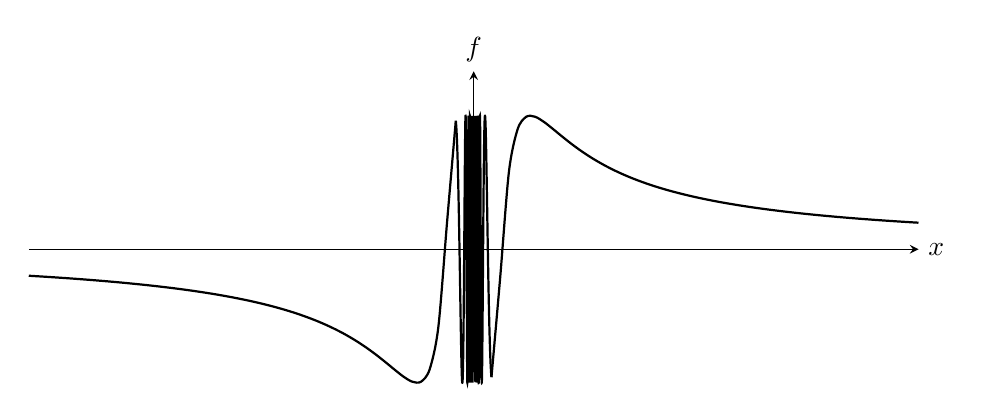
\begin{tikzpicture}[scale=1.13, >=stealth]
        \draw[->] (-5, 0) -- (5, 0) node[right] {$x$};
        \draw[->] (0, -0.8) -- (0, 2) node[above] {$f$};

        \def\functionplot{plot (\x,{1.5 * sin((1/\x) r)})}
        \draw[thick, domain=0.01:0.2, samples=1000] \functionplot;
        \draw[thick, domain=0.2:5, smooth, samples=50] \functionplot;
        \draw[thick, domain=-0.2:-0.01, samples=1000] \functionplot;
        \draw[thick, domain=-5:-0.2, smooth, samples=50] \functionplot;
      \end{tikzpicture}
    \end{center}

      Consider the sequence $(x_n)$ on $\R$ given by:
      \[
        x_n = \frac{1}{(2n + \frac{1}{2})\pi}
      \]
      $x_n \to 0$, so if $f$ is sequentially continuous, then we would expect $f(x_n) \to 0$.
      However, $f(x_n) = \sin((2n + \frac{1}{2})\pi) = 1\ \forall n \implies f(x_n) \to 1$ and so $f$ is not sequentially continuous and therefore also not continuous.
    \item The \textit{Dirichlet function}:
      \[
        f(x) = 1_\Q(x) = \begin{cases}
        1 & \text{ if } x \in \Q \\
        0 & \text{ if } x \notin \Q
        \end{cases}
      \]
      is discontinuous at every point in $\R$.

      \begin{itemize}
        \item For $a \in \Q$, there exists a sequence $(x_n)$ on $\R$ with $x_n \to a$.
          But $f(x_n) = 0\ \forall n \implies f(x_n) \to 0$ but $0 \neq 1 = f(a)$ and so $f$ is not continuous at $a$.
        \item For $a \in \R \setminus \Q$, there exists a sequence $(x_n)$ on $\R \setminus \Q$ with $x_n \to a$.
          But $f(x_n) = 1\ \forall n \implies f(x_n) \to 1$ but $1 \neq 0 = f(a)$ and so $f$ is not continuous at $a$
      \end{itemize}
      Therefore it is not continuous for all points in $\Q \cup (\R \setminus \Q) = \R$.

      This can also be shown using the non sequential definition of continuity, again utilising that both irrational and rational numbers are dense in the reals.
  \end{enumerate}
\end{example}
\subsection{Continuity Properties}
\begin{lemma}[Continuity Laws]
  If $f, g: X \subseteq \C \to \C$ are continuous at $a \in X$, then so are:
  \label{continuityLaws}
  \begin{enumerate}
    \item $\lambda f + g$ for fixed $\lambda \in \C$
    \item $fg$
    \item $\frac{1}{f}$ provided that $f(z) \neq 0\ \forall z \in X$.
  \end{enumerate}
\end{lemma}
\begin{proof}
  Since $f$ and $g$ are continuous at $a$, $\forall \varepsilon > 0$:
  \begin{align*}
    \exists \delta_1 = \delta_1(\varepsilon) \text{ s.t. } |z - a| < \delta_1 \implies |f(z) - f(a)| < \varepsilon \\
    \exists \delta_2 = \delta_2(\varepsilon) \text{ s.t. } |z - a| < \delta_2 \implies |g(z) - f(a)| < \varepsilon
  \end{align*}
  \begin{enumerate}
    \item $\forall z \text{ s.t. } |z - a| < \min\{\delta_1, \delta_2\}$, we have:
      \begin{align*}
        |\lambda f(z) + g(z) - \lambda f(a) - g(a)| &\leq |\lambda||f(z) - f(a)| + |g(z) - g(a)| \\
                                                    &< \varepsilon(|\lambda| + 1)
      \end{align*}
      This is a constant multiple of $\varepsilon$, so $\lambda f + g$ is continuous at $a$.
    \item We can also pick $\varepsilon = 1$ so that:
      \[
        \exists \delta_3 \text{ s.t. } |z - a| < \delta_3 \implies |f(z) - f(a)| < \varepsilon \implies |f(z)| < 1 + |f(a)|
      \]
      Then $\forall z \text{ s.t. } |z - a| < \min\{\delta_1, \delta_2, \delta_3\}$:
      \begin{align*}
        |f(z)g(z) - f(a)g(a)| &= |f(z)g(z) - f(z)g(a) + f(z)g(a) - f(a)g(a)| \\
                        &\leq |f(z)||g(z) - f(a)| + |g(a)||f(z) - f(a)| \\
                        &< (1 + |f(a)|)\varepsilon + |g(a)|\varepsilon \\
                        &= \varepsilon(1 + |f(a)| + |g(a)|)
      \end{align*}
      which is a constant multiple of $\varepsilon$, so $fg$ is continuous at $a$.
    \item We can pick $\varepsilon = \abs{\frac{f(a)}{2}} > 0$ so that:
      \[
        \exists \delta_3 \text{ s.t. } |z - a| < \delta_3 \implies |f(z) - f(a)| < \abs{\frac{f(a)}{2}} \implies |f(z)| > \abs{\frac{f(a)}{2}} > 0
      \]
      Then $\forall z \text{ s.t. } |z - a| < \min\{\delta_1, \delta_2, \delta_3\}$:
      \begin{align*}
        \abs{\frac{1}{f(z)} - \frac{1}{f(a)}} &= \frac{1}{|f(a)||f(z)|}|f(z) - f(a)| \\
                                       &< \frac{\varepsilon}{|f(a)||\frac{f(a)}{2}|}
      \end{align*}
      which is a constant multiple of $\varepsilon$, so $\frac{1}{f}$ is continuous at $a$.
  \end{enumerate}
\end{proof}
\begin{remark}
  The above proof is very similar to the proof of limit laws in \cref{limitLaws}.
\end{remark}
Function composition also preserves continuity.
\begin{lemma}[Continuity Under Composition]
  Let $U, V \subseteq \C$ and $f: U \to V$ and $g: V \to \C$.
  If $f$ is continuous at $a \in U$ and $g$ is continuous at $f(a) \in V$, then $g \circ f: U \to \C$ is continuous at $a$.
\end{lemma}
\begin{proof}
  For arbitrary $\varepsilon > 0$, since $g$ is continuous at $f(a)$:
  \[
    \exists \delta_1 = \delta_1(\varepsilon) \text{ s.t. } |y - f(a)| < \delta_1 \text{ for } y \in V \implies |g(y) - g(f(a))| < \varepsilon
  \]
  Since $f$ is continuous at $a$, using $\delta_1$ in place of $\varepsilon$ in the definition:
  \[
    \exists \delta_2(\delta_1) = \delta_2(\varepsilon) \text{ s.t. } |z - a| < \delta_2 \text{ for } z \in U \implies |f(z) - f(a)| < \delta_1
  \]
  Bringing this all together, $\forall \varepsilon > 0$:
  \begin{align*}
    \exists \delta_2 = \delta_2(\varepsilon&) \text{ s.t. } |z - a| < \delta_2 \text{ for } z \in U \\
    &\implies |f(z) - f(a)| < \delta_1 \text{ for $f(z) \in V$} \\
    &\implies |g(f(z)) - g(f(a))| < \varepsilon
  \end{align*}
  Thus, $g \circ f$ is continuous at $a$.
\end{proof}
\section{Extreme Value Theorem}
\begin{definition}[Closed Set]
  A set $X \subseteq \C$ is \textit{closed} if all the sequences $(x_n)$ in $X$ which converge in $\C$ have their limit in $X$.
\end{definition}
\begin{remark}
  We use this definition here as it applies to $\C$ and any arbitrarily defined set, however, it is often useful to relate this definition to the real interval $[a, b]$ because that is what we will be primarily using.
\end{remark}
\begin{example}
  The interval $[0, 1]$ is closed whereas the interval $(0, 1)$ is not.
  Neither are mixed intervals like $[0, 1)$ or $(0, 1]$.

  Intervals with infinite endpoints can be closed, for example, $[0, \infty)$ is closed while $(0, \infty)$ is not.
\end{example}
\begin{definition}[Bounded Set]
  A set $X \subseteq \C$ is \textit{bounded} if there exists $\exists M > 0$ such that:
  \[
    X \subseteq \{z \in \C: |z| \leq M\}
  \]
  or equivalently, if $\exists M > 0$ such that:
  \[
    \sup_{z \in X} |z| \leq M
  \]
\end{definition}
\begin{example}
  The intervals $[0, 1], (0, 1), [0, 1), [0, 1]$ are all bounded but $[0, \infty)$ and $(0, \infty)$ are not bounded.
\end{example}
\begin{proposition}[Continuity Preserves Bounded Closed Sets]
  Let $X \subseteq \C$ be a bounded closed set.
  If $f: X \to \C$ is continuous, then $f(X) \subseteq \C$ is also a bounded closed set.
  \label{boundedClosedPreserved}
\end{proposition}
\begin{proof}\par
  \textbf{$f(X)$ is bounded}\par
  For the purposes of contradiction, suppose $f(X)$ is not bounded, then for each $n \in \N$, we can find $x_n \in X$ such that $|f(x_n)| > n$.
  We can use this to construct a sequence $(x_n)$ on $X$.
  $X$ is bounded by assumption so the sequence must also be bounded.
  This means that we can apply the Bolzano Weierstrass theorem (\cref{BWT}), so there exists a convergent subsequence $(x_{n_k})$ where $x_{n_k} \to x$ for some $x \in \C$.
  Since $X$ is closed, all convergent sequences in $X$ must converge to a value in $X$ and so $x \in X$.

  On the other hand, $|f(x_{n_k})| > n_k \geq k$ since $n_k$ is strictly increasing.
  Thus $f(x_{n_k})$ cannot converge as $k \to \infty$.
  This contradicts the sequential continuity of $f$ (\cref{sequentialContinuity}) as $x \in X$ and so $f(X)$ must be bounded.

  \textbf{$f(X)$ is closed}\par
  Take any convergent sequence $(y_n)$ in $f(X)$ and suppose that it converges to some $y \in \C$.
  By definition, to show that $f(X)$ is closed, we need to show that $y \in f(X)$.

  Since $y_n \in f(X)$, $\exists x_n \in X$ such that $f(x_n) = y_n$.
  Similarly to before, we can use this construct a sequence $(x_n)$ in $X$.
  Since $X$ is bounded, $(x_n)$ must also be bounded and so as in the previous argument, we can construct a sequence $x_{n_k} \to x \in X$.
  $f$ is continuous by assumption so:
  \[
    \lim_{k \to \infty} f(x_{n_k}) = f\left(\lim_{k \to \infty} x_{n_k}\right) = f(x)
  \]
  Therefore, $y_{n_k} = f(x_{n_k}) \to f(x) \in f(X)$ and so $(y_{n_k})$ converges to a limit in $f(X)$.
  Since $y_n \to y$ and all subsequences must converge to the same limit (\cref{subseqenceConvergence}), we have $y = f(x) \in f(X)$, which is the required result.
\end{proof}
\begin{theorem}[Extreme Value Theorem]
  Let $X \subseteq \R$ be a bounded closed set.
  If $f: X \to \R$ is continuous, then $\exists a, b \in X$ such that:
  \[
    f(a) = \sup f(X) = \sup_{z \in X} f(z),\ f(b) = \inf f(X) = \inf_{z \in X} f(z)
  \]
\end{theorem}
\begin{remark}
  We know from \cref{boundedClosedPreserved} that $f(X)$ must be bounded so by the axioms of the real numbers there always exists supremum and infimum for $f(X)$.
  The important distinction of the extreme value theorem is that it shows us that such values are actually attained and so they are really maximum and minimum of $f(X)$.
\end{remark}
\begin{proof}
  We will prove the first equality as the other is proved analogously.

  By \cref{boundedClosedPreserved}, $f(X)$ is closed and bounded so we can let $M = \sup f(X)$.
  By definition of supremum $M - \frac{1}{n}$ cannot be an upper bound for $f(X)$ for any $n \in \N$.
  Therefore, for each $n$, there exists $y_n \in f(X)$ such that $M - \frac{1}{n} < y_n \leq M$.
  We can use this to construct a sequence $(y_n)$ on $f(X)$.

  Taking limits, $M \leq \lim_{n \to \infty} y_n \leq M$ and so $y_n \to M$.
  Since $f(X)$ is closed, $M \in f(X)$ and so $\sup f(X) \in f(X) \implies \exists a \in X \text{ s.t. } f(a) = \sup f(X)$ as required.
\end{proof}
\section{Intermediate Value Theorem}
\begin{theorem}[Intermediate Value Theorem]
  If $f: [a, b] \to \R$ is continuous and WLOG, then given any $y$ between $f(a)$ and $f(b)$ there exists $c \in [a, b]$ such that $f(c) = y$.
  \label{IVT}

  More generally, $f([a, b])$ is a closed interval containing the interval:
  \[
    [\min\{f(a), f(b)\}, \max\{f(a), f(b)\}]
  \]
\end{theorem}
\begin{remark}
  Although this guarantees the existence of such a $c$, it is not necessarily unique as there could be multiple points whose image is $y$.
\end{remark}
\begin{proof}
  If $f$ is constant or $y \in \{f(a), f(b)\}$, then the result follows trivially, if not, assume WLOG that $f(a) < y < f(b)$.

  Consider the set $S = \{x \in [a, b]: f(x) \leq y\}$.
  $a \in S$ so $S \neq \emptyset$.
  $S$ is also bounded above by $b$ so $\exists d = \sup S \in [a, b]$.
  It would be reasonable to guess that $d$ is a point satisfying $f(d) = y$.
  To show this, we can show both $f(d) \leq y$ and $f(d) \geq y$.

  \textbf{Claim $f(d) \leq y$}\par
  Suppose, for contradiction, that $f(d) > y$.
  We can then pick $\varepsilon = f(d) - y > 0$ and so by continuity of $f$, $\exists \delta > 0 \text{ s.t. } |x - d| < \delta \text{ for $x \in [a, b]$} \implies |f(x) - f(d)| <\varepsilon$.
  We also have that:
  \[
    |f(x) - f(d)| < \varepsilon \iff - \varepsilon < f(x) - f(d) < \varepsilon \implies f(x) > f(d) - \varepsilon = y \implies x \notin S
  \]
  So $\forall x \in [a, b] \text{ s.t. } |x - d| < \delta \implies x \notin S$, therefore $S \cap (d - \delta, d) = \emptyset$ which contradicts that $d$ is the supremum of $S$.

  \textbf{Claim $f(d) \geq y$}\par
  Suppose, for contradiction, that $f(d) < y$.
  We can then pick $\varepsilon = y - f(d) > 0$.
  By continuity of $f$, $\exists \delta > 0 \text{ s.t. } |x - d| < \delta \text{ for $x \in [a, b]$} \implies |f(x) - f(d)| < \varepsilon$.
  We also have that:
  \[
    |f(x) - f(d)| < \varepsilon \iff - \varepsilon < f(x) - f(d) < \varepsilon \implies f(x) < f(d) + \varepsilon = y
  \]
  However, if we consider $x = d + \frac{\delta}{2}$, $|d + \frac{\delta}{2} - d| < \varepsilon \implies f(d + \frac{\delta}{2}) < y$ and so $d + \frac{\delta}{2} \in S$ but $d + \frac{\delta}{2} > d$ which contradicts the fact that $d$ is an upper bound for $S$.

  \textbf{Intervals}\par
  For the more general statement, let $I = [a, b]$ and $J = f([a, b])$ and take any $y_1, y_2 \in J$.
  Since $y_1, y_2 \in f(I)$, there exists $x_1, x_2 \in I$ with $f(x_1) = y_1$ and $f(x_2) = y_2$.

  Since $[a, b]$ is an interval, $x_1, x_2 \in I \implies [x_1, x_2] \subseteq I$.
  By the above, given $y$ between $y_1$ and $y_2$, there exists a $c \in [x_1, x_2]$ such that $y = f(c) \in f(I) = J$.
  Therefore, any point between $y_1$ and $y_2$ is also in $J$ and so $J$ is an interval.
  Finally, $f(a) \in J$ and $f(b) \in J$ so:
  \[
    [\min\{f(a), f(b)\}, \max\{f(a), f(b)\}] \subseteq J
  \]
  since $J$ is an interval.
\end{proof}
\begin{example}[$n$-th Roots]
  We can apply the intermediate value theorem to show the existence of $n$-th roots.

  Take $t > 0$ and consider $f: [0, 1 + t] \to \R, x \mapsto x^{N}$ for some $N \in \N$.
  This is a continuous function and since $(1 + t)^{N} \geq t$ using binomial theorem, we have:
  \[
    0 = f(0) < t < (1 + t)^{N} = f(1 + t)
  \]
  Applying the intermediate value theorem, we conclude that $\exists c \in [0, 1 + t]$ such that $f(c) = t \iff c^{N} = t$.
  Hence $c$ is an $N$-th root of $t$.
\end{example}
\begin{definition}[Monotone Function]
  We say that a function $f: [a, b] \to \R$ is \textit{monotone} if either:
  \begin{itemize}
    \item It is \textit{increasing}: $a \leq x_1 \leq x_2 \leq b \implies f(x_1) \leq f(x_2)$.
    \item It is \textit{decreasing}: $a \leq x_1 \leq x_2 \leq b \implies f(x_1) \leq f(x_2)$.
  \end{itemize}
\end{definition}
\begin{remark}
  A function is \textit{strictly increasing} if:
  \[
    a \leq x_1 < x_2 \leq b \implies f(x_1) < f(x_2)
  \]
  and \textit{strictly decreasing} if:
  \[
    a \leq x_1 < x_2 \leq b \implies f(x_1) > f(x_2)
  \]
\end{remark}
\begin{proposition}[Inverse function theorem for monotone functions]
  Let $f: [a, b] \to \R$ be a continuous function that is strictly decreasing or strictly increasing and let $c = \min\{f(a), f(b)\}, d = \max\{f(a), f(b)\}$.

  Then $f: [a, b] \to [c, d]$ is a bijection and there exists a continuous inverse $f^{-1}: [c, d] \to [a, b]$ which is strictly increasing if $f$ is and strictly decreasing if $f$ is.
\end{proposition}
\begin{proof}\par
  WLOG assume that $f$ is strictly increasing as if it was strictly decreasing, we can just use the strictly increasing case on $-f$.
  \textbf{Bijection --} Since $f$ is strictly monotone, it maps $[a, b] \to [c, d]$ as the extreme values must occur at the endpoints of the codomain.
  Since it is strictly monotone, it must also be injective.

  It is also surjective by the intermediate value theorem (\cref{IVT}) as for any $y \in [c, d]$, there exists $c \in [a, b]$ such that $f(c) = y$.

  \textbf{Strictly Monotone --}

  Suppose $f^{-1}: [c, d] \to [a, b]$ is not strictly increasing, then $\exists y_1, y_2 \in [c, d]$ with $y_1 < y_2$ but $f^{-1}(y_1) \geq f^{-1}(y_2)$.

  Since $f$ is strictly increasing, it preserves inequalities and so $f(f^{-1}(y_1)) \geq f(f^{-1}(y_2))$.
  But we now know that $f$ is a bijection so this implies that $y_1 \geq y_2$ which is a contradiction, thus $f^{-1}$ must be strictly increasing.

  \textbf{Continuity --} Consider a fixed $y_0 \in [c, d]$ and let $x_0 = f^{-1}(y_0)$.
  There are three cases to consider as we need to ensure that adding or subtracting $\delta$ does not cause us to stray outside the domain of $f$.
  \begin{proofcases}
    \begin{case}{$x_0 \in (a, b)$}
      Since $(a, b)$ does not include its endpoints, for fixed $\varepsilon > 0$, we can choose $\eta \in (0, \varepsilon]$ to be sufficiently small so that $[x_0 - \eta, x_0 + \eta] \subseteq [a, b]$.
      Since $f$ is strictly increasing, applying $f$ preserves inequalities so:
      \[
        x_0 - \eta < x_0 < x_0 + \eta \implies f(x_0 - \eta) < y_0 < f(x_0 + \eta)
      \]

      We can use this inequality to construct two positive quantise that we can try to use as a $\delta$:
      \[
        \delta(\varepsilon) = \min\{f(x_0 + \eta) - y_0, y_0 - f(x_0 - \eta)\}
      \]
      Then, to show continuity, consider:
      \begin{align*}
        |y -  y_0| < \delta,\ y \in [c, d] &\implies y_0 - \delta < y < y_0 + \delta \\
                                           &\implies f(x_0 - \eta) \leq y_0 - \delta < y < y_0 + \delta \leq f(x_0 + \eta) \\
                                           &\implies f(x_0 - \eta) < y < f(x_0 + \eta) \\
                                           &\implies x_0 - \eta < f^{-1}(y) < x_0 + \eta \\
                                           &\implies |f^{-1}(y) - x_0| < \eta < \varepsilon \\
                                           &\implies |f^{-1}(y) - f^{-1}(y_0)| < \varepsilon
      \end{align*}
      Thus $f^{-1}(y)$ is continuous at $y_0$.
    \end{case}
    \begin{case}{$x_0 = a$}
      For fixed $\varepsilon > 0$, we choose $\eta = \min\{\varepsilon, b - a\}$ so that $a + \eta \in [a, b]$.
      Since $f$ is strictly monotone increasing, $f(a + \eta) > f(a) \implies f(a + \eta) - f(a) > 0$ so we can set $\delta(\eta) = f(a + \eta) - f(a)$.

      To show continuity, we can utilise the fact that because $a = \min [a, b]$ and $f$ is monotone increasing $y \geq f(a) = y_0\ \forall y \in [c, d]$
      \begin{align*}
        |y - y_0| < \delta,\ y \geq y_0 &\implies y_0 \leq y < y_0 + \delta = f(a) + \delta \\
                                        &\implies f(a) \leq f(a) + \delta = f(a + \eta) \\
                                        &\implies a \leq f^{-1}(y) \leq a + \eta \\
                                        &\implies |f^{-1}(y) - a| < \eta \leq \varepsilon \\
                                        &\implies |f^{-1}(y) - f^{-1}(y_0)| \leq \varepsilon
      \end{align*}
      and so $f^{-1}(y)$ is continuous at $y_0$.
    \end{case}
    \begin{case}{$x_0 = b$}
      This case is performed analogously to $x_0 = a$ apart from now $\eta = \min\{\varepsilon, b - a\}$ ensures that $b - \eta \in [a, b]$ and we utilise the fact that $y \leq y_0\ \forall y \in [c, d]$.
    \end{case}
  \end{proofcases}
  So $f^{-1}$ is continuous at any $y_0 \in [c, d]$ and so $f^{-1}$ is continuous over its domain.
\end{proof}
\end{document}
